\documentclass[conference,10pt]{IEEEtran}
%\documentclass[conference,draft,onecolumn]{IEEEtran}
% useful packages, copy and paste from diff sources

\usepackage[english]{babel}
\usepackage[T1]{fontenc}
\usepackage{cite,url,color} % Citation numbers being automatically sorted and properly "compressed/ranged".
\usepackage{graphics,amsfonts}
\usepackage{epstopdf}
\usepackage[pdftex]{graphicx}
\usepackage[cmex10]{amsmath}
\usepackage[flushleft]{threeparttable}
\usepackage{etoolbox}
\usepackage{adjustbox}
\usepackage{multirow}
\usepackage{breqn}

% Also, note that the amsmath package sets \interdisplaylinepenalty to 10000
% thus preventing page breaks from occurring within multiline equations. Use:
\interdisplaylinepenalty=2500
% after loading amsmath to restore such page breaks as IEEEtran.cls normally does.
\usepackage[utf8]{inputenc}
% Useful for displaying quotations
%\usepackage{csquotes}
% Compact lists
%\let\labelindent\relax
\usepackage{enumitem}

%tikz figures
\usepackage{tikz}
\usetikzlibrary{automata,positioning,chains,shapes,arrows}
\usepackage{pgfplots}
\usetikzlibrary{plotmarks}
\newlength\fheight
\newlength\fwidth
\pgfplotsset{compat=newest}
\pgfplotsset{plot coordinates/math parser=false}

\usepackage{array}
% http://www.ctan.org/tex-archive/macros/latex/required/tools/
%\usepackage{mdwmath}
%\usepackage{mdwtab}
%mdwtab.sty	-- A complete ground-up rewrite of LaTeX's `tabular' and  `array' environments.  Has lots of advantages over
%		   the standard version, and over the version in `array.sty'.
% *** SUBFIGURE PACKAGES ***
%\usepackage[tight,footnotesize]{subfigure}
\usepackage{subfig}

\usepackage[top=1.5cm, bottom=2cm, right=1.6cm,left=1.6cm]{geometry}
\usepackage{indentfirst}

\usepackage{times}
% make sections titles smaller to save space
%\usepackage{sectsty}
%\sectionfont{\large}
% enable the use of 'compactitem', a smaller 'itemize'
%\usepackage{paralist}

% MP
% to split equations using dmath env
\usepackage{breqn}
% nice rules in tables
\usepackage{booktabs}

%\setlength\parindent{0pt}
\linespread{1}

% MC
\newcommand{\TD}[1]{\textit{\color{blue}DT says: #1}}
\newcommand{\AZ}[1]{\textit{\color{red}AZ says: #1}}
\newcommand{\MP}[1]{\textit{\color{green}MP says: #1}}

\usepackage{placeins}


%%%%%%%%%%%%%%%%%%%%%%%%%%%%%%%%%%%%%%%%%%
\begin{document}
%%%%%%%%%%%%%%%%%%%%%%%%%%%%%%%%%%%%%%%%%%
\title{Self-Organizing Networks	in LTE: a Q-learning approach to ABS optimization}

\author{\IEEEauthorblockN{Andrea Maracani, Marco Rossanese, Davide Talon}
\IEEEauthorblockA{Department of Information Engineering, University of Padova -- Via Gradenigo, 6/b, 35131 Padova, Italy\\Email: {\tt\{andrea.maracani,marco.rossanese,davide.talon\}@studenti.unipd.it}
}}

\maketitle
\thispagestyle{plain}
\pagestyle{plain}
\begin{abstract}
In this paper we introduce a possible machine-learning approach for the enhanced inter-cell interference coordination (eICIC) in a heterogeneous network (HetNet), where macro and micro cells optimize their downlink transmission in a self-adaptive manner. The idea is to exploit the Q-learning algorithm to guarantee a fair resource sharing between micro and macro cells and so to make the system works in the best performance possible. Indeed this specific reinforcement learning technique is used to find out the optimal policy that leads to the right ABS pattern setting, designed specifically for each scenario. Hence evaluating only a few parameters and changing dynamically the ABS pattern we aim to cope the possible alterations on a realistic environment.\TD{Results preview}\\

\textit{Index  Terms}---SON, Self Optimizing Networks, LTE, eICIC, ABS, reinforcement learning, Q-learning, MONSTeR     
\end{abstract}

%%%%%%%%%%%%%%%%%%%%%%%%%%%%%%%%%%%%%%%%%
\section{Introduction}\label{sec:intro}
%%%%%%%%%%%%%%%%%%%%%%%%%%%%%%%%%%%%%%%%%
The great spreading of mobile devices all over the world represents the fastest adoption of any technology that
our society has ever experienced, faster than the Internet and the earlier generations of mobile
communications. Now tablets, android devices, iPhones, application stores, social media and the data
exchanges between end-users and clouds are all growing at exponential speed. Providing the necessary bandwidth and capacity to the people so they can keep the pace of this growth is a fascinating challenge; in order to achieve that, an increased network densification is required together to a full exploitation of the simultaneous presence of micro (coverage radius around 10m-300m) and macro (coverage radius up to 20km) cells, the so called heterogeneous networks (HetNet). Figure \ref{img:hetnet} illustrates a typical HetNet configuration.\\
In 2016, global mobile data traffic amounted to 7 exabytes (EB)\footnote{1 EB = $8\cdot 10^{18}$ bit} per month; in 2021, mobile data traffic worldwide is expected to reach 49 exabytes per month at a compound annual growth rate of 47 percent \cite{indexglobal}.
These challenges can be solved in a cost-effective, efficient and human-handleable way only through the use of more automated and autonomous systems, such as Self-Organizing Networks (SON): the goal is to minimize the human intervention in the planning, deployment, optimization and maintenance activities of these new networks.\\
Such a SON conceptually must own, as explained by \cite{ramiro2011self}, the following capabilities:
\begin{itemize}
\item Self-Planning: process of identifying the parameter settings of new network elements (like radio parameters of a new eNodeB or a table of neighbour nodes);
\item Self-Deployment: preparation, installation, authentication and delivery of a status report of
a new network node in order to get a "plug and play" approach for each new device;
\item Self-Healing: execution of the routine actions that keep the network operational and/or
prevent problems (this includes the necessary software and hardware upgrades);
\item Self-Optimization is defined as the utilization of measurements and performance indicators
collected by the User Equipments (UEs) and the base stations in order to auto-tune the network
settings.
\end{itemize}
Our work is focused on the last point of the list, more precisely on the improvement of the signal quality and consequently the throughput in a LTE system, trying to minimize the interference between micro and macro cells with an adaptive coordination in downlink transmissions of the antennas (mainly controlling the transmit power patterns).\\
The problem we are facing consists in finding the optimal trade-off between assigning the radio resources to high-power nodes (macro) or low-power nodes (micro). The latter has an higher capacity and consequently an user connected to it will have better performances; however, low-power nodes are severely affected by the interference from the high-power nodes, due to fact that they share the same frequency band with the macro. In other words, downlink micro transmissions to its UEs could be sorely degraded by high power macro transmission; besides UEs that are close to a micro could end up associating to a macro due to the higher power strength received from the stronger node.\\
Accounting the above scenario, the micro could be left underutilized and this would turn out to be a bad exploitation of the resources deployed appositely to enhance the connectivity in some areas, with a following shortage of the user performance in comparison with achievable potential capacity.\\
Addressing a fair resource sharing, a solution could be stop macros from all the transmissions (some exception signals, like beacons, are always active), for a certain amount of time: this approach is adopted by LTE 3GPP standard and it is known as enhanced Inter Cell Interference Coordination (eICIC). The period in which macros are "silent" is called Almost Blank Subframe (ABS), period over which micros can transmit with reduced interference.\\
Time is slotted in frames of 10 ms and each one of these is split into 10 subframes, so a macro decides to mute itself in a certain subframe following the ABS mask, that's the pattern of 0's and 1's where 1 indicates the macro's inactivity.\\
The goal is to discover an adaptive ABS mask that maximizes the UEs' performance and it is found as the result of an optimization problem. Our idea is to use a reinforcement learning (RL) approach, the Q-learning technique, in order to reach the fairness between the shared resources and to set the best ABS mask in a self-tuning manner for each specific scenario.\\
Thanks to the LTE environment simulator MONSTeR (MObile Networks SimulaToR) \cite{monster}, a framework built around the LTE system toolbox available in MATLAB, we simulate a great amount of data traffic with the purpose of training the Q-learning: after this period the method involved will yield the best policy for setting the considered mask.
\begin{figure}[h]
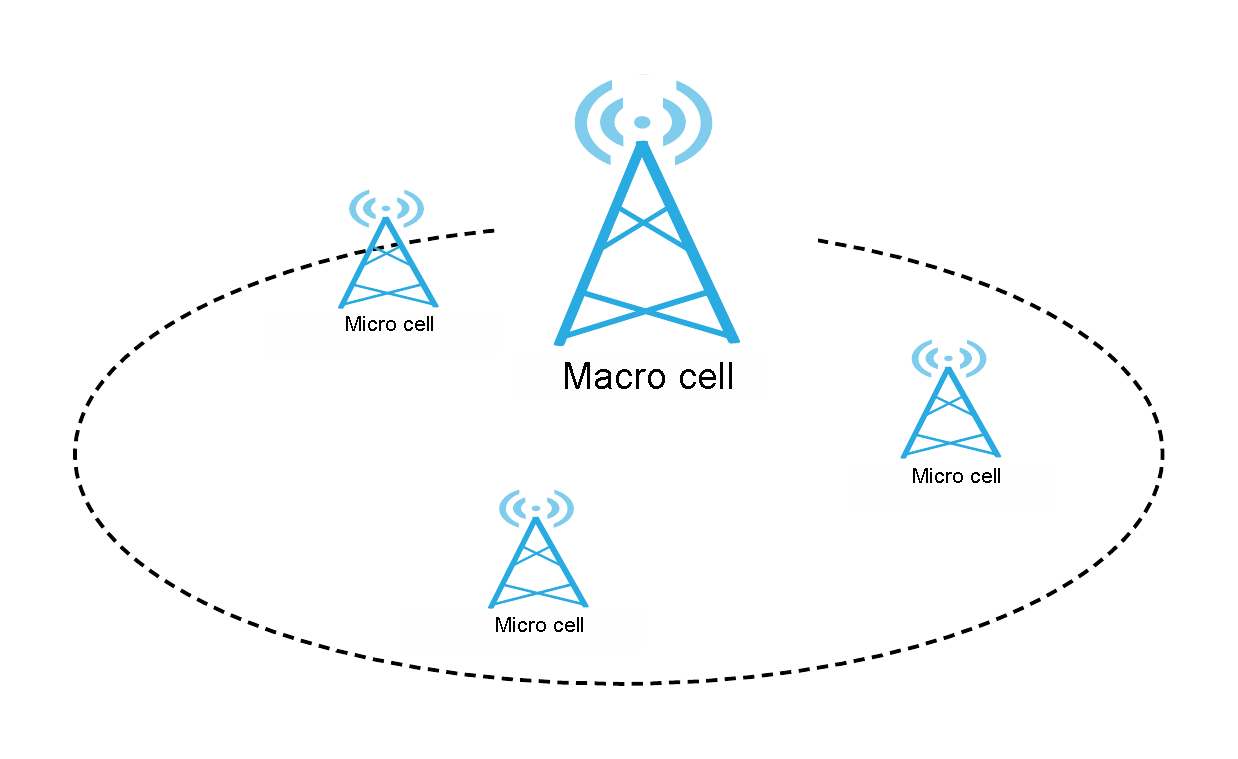
\includegraphics[scale=0.80]{figures/ABS.png}
\caption{Example of a typical HetNet with a macro and some micros used for throughput enhancement in high density utilization area; a micro is placed on the edge of the coverage area for improving throughput of the border UEs. }\label{img:hetnet}
\end{figure}     


\textcolor{red}{
\textbf{TO DO (REMEMBER TO ERASE THIS)}
\begin{itemize}
\item \textbf{Results: summary of the main findings}
\end{itemize}}

The rest of the paper is organized as follows: Section II
presents how eICIC is addressed in literature. Section III introduces the system
model, specifying the necessary theoretical background to explain the steps that leaded us to define it. 
Section IV states all the simulation settings adopted for the environment and testing scenario; finally Section V  concludes the work analyzing the achieved results and comparing the obtained policy with benchmark ones.


%%%%%%%%%%%%%%%%%%%%%%%%%%%%%%%%%%%%%%%%%%%%
\section{Related Work}\label{sec:sota}
%%%%%%%%%%%%%%%%%%%%%%%%%%%%%%%%%%%%%%%%%%%%
In this section we will overview the main proposals in the literature.\\
First of all we must take in account the solution exposed in \cite{deb2014algorithms} to protect the downlink micro transmissions. Alongside the concept of ABS period they introduced the so called Flexible User Association and Cell selection bias (CSB). As we already know, whenever a UE needs to select a suitable cell for association it chooses the one with the strongest signal and therefore the utilization of the micro most of the time is neglected. LTE has introduced the bias value $\alpha_i$ that is broadcasted to all the UEs. Hence the UE will choose the right cell maximizing the sum between $\alpha_i$ and the received signal power $P_i$ over each i-th cell in the system; obviously higher bias values are assigned to the micros.\\
Deb \textit{et al.}\cite{deb2014algorithms} proposed two algorithms, one for the optimal ABS mask (OPT-ABS) and one for defining the right value for the CBS. The former is split into two parts: the first to search the number of optimal subframes in which the macros are mute and second how to define the optimal ABS pattern. This algorithm turned up to be a NP-hard computational problem, however they proofed that with a clever breakdown in some defined steps it's implementable and the complexity is scalar with number of cells. Instead the latter algorithm compute the biases so that the "association error" (as compared to optimal association) is minimized. This technique shows a shortcoming since that the beforehand knowledge of the best cell is an information not always available and so it needs to be evaluated for each scenario.\\
Another noteworthy paper is surely \cite{simsek2013enhanced}, here the authors tried to put into practice a similar reinforcement learning approach. The state is made of two parameters, the Signal to Intererence Noise Ratio (SINR) for the player in relation with the macro and the micros, nevertheless these are not values that the eNodeB takes normally into account and we are aiming to use only the minimum number of information that are already exchanged (all the info shared between eNodeB and UE are listed in the 3GPP release 36 \cite{etsi2017136}) reducing the system overhead. 

%%%%%%%%%%%%%%%%%%%%%%%%%%%%%%%%%%%%%%
\section{System Model}\label{sec:symo}
%%%%%%%%%%%%%%%%%%%%%%%%%%%%%%%%%%%%%%
In this section we will explain all the operative assumptions, with the theoretical motivations, that we took into account for our proposal.
\subsection{Problem modelization}
As stated in \cite{sutton1998reinforcement}, the main book about RL: the reinforcement learning problem is meant to be a straightforward framing of the problem of learning from interaction to achieve a goal. The learner, who is the one that makes the decisions is called the agent and in this scenario will be the macro. The thing it interacts with, comprising everything outside the agent, is called the environment, part played here by the simulator MONSTeR. These interact continually, the agent selecting actions and the environment reacting to those actions and presenting new situations to the agent. The environment also yields rewards, numerical values that evaluate the goodness of the last action taken and that the agent tries to maximize over time. Defining $S$ as the set of all possible states and $A_s$ as the available actions at state $s$, the problem is modelled as a finite Markov Decision Process (MDP) defined as a 5-tuple:
\begin{equation*}
(S, A_s, P_a(s_t, s_{t+1}), R_a(s_t, s_{t+1}), \gamma)
\end{equation*}
where $P_a(s_t, s_{t+1})$ represents the probability to move from state $s_t$ to state $s_{t+1}$ with action $a \in A_s$, $R_a(s_t, s_{t+1})$ describes the obtained reward from the transaction $s_t$ towards $s_{t+1}$ with action $a_t \in A_s$ and the discount factor $\gamma$ reflects how to weight future actions' reward. Therefore the environment is represented as a Markov chain in which each transaction relies on the agent's action and environment's response. We need a small as possible state space to reduce the complexity of the MDP, but at the same time each state should contains
enough information to preserve the Markov's property. Hence, at each time step $t$, the agent receives a representation of the environment's state $S_t$, here defined by three parameters:
\begin{itemize}
\item the ratio between the number of users in the macro and in the micro, quantized in four values which indicates if there are many more users in the macro, a little bit more in the macro, a little bit more in the micro or many more in the micro;
\item the ratio between the throughput of the macro cell and the mean value of the throughtput of all micro cells, quantized in five values;
\item the number of ABS is quantized in six values where each of them stays for the amount of subframes in which the macro cell stays silent. In particular we just consider ABS masks composed by an even number of silent subframes, that are actually six.
\end{itemize}
Then, for the curse of dimensionality, the total number of possible states in our environment is exactly $4\cdot 5\cdot 6=120$ which allow us to handle the convergence problem. Depending in which state the agent is, it selects an action $A_t$ from the set of all actions $A=\lbrace-2,0,2\rbrace$ that will modify the ABS mask by this amount. In the states where the ABS mask is equal to 0 there is not the decreasing-action (-2) and in the states with ABS mask equal to 10 there is not the increasing action (+2). The reward is a number between 0 and 10 and it must be an high value when the ratio between the thoughput per user in the macro cell and the throughput per user in the microcells is close to one. In fact this condition is index of fairness between the downlink transmissions for users in the macro cell and users in the micro cells. In particular the ratio we consider is: 
\begin{equation*}
r(n^{m},n^{M},S^{m},S^{M})=\bigg(\frac{ S^{M} / n^{M} }{S^{m} / n^{m}} \bigg)= \bigg(\frac{ S^{M} \cdot n^{m}}{S^{m} \cdot n^{M}} \bigg)
\end{equation*}
And so, the reward function we consider is:
\begin{dmath*}
Reward(n^{m},n^{M},S^{m},S^{M}) = \begin{cases} 10 \cdot r(n^{m},n^{M},S^{m},S^{M}), & \mbox{if } r<1 \\ max( 10 \cdot(2 - r(n^{m},n^{M},S^{m},S^{M}),0), & \mbox{if } r>1 \end{cases}
\end{dmath*} 
where $m$ stands for micro and $M$ for macros and it shows the discrepancy between the actual system condition and the equilibrium we're aiming to. \\
At each time step, the agent maps from states to probabilities of taking each possible action. This mapping is called policy and is denoted as $\pi:S \times S \times A \rightarrow R$. Reinforcement
learning specifies how the agent changes its policy in relation of its experience. The agent's goal is to learn actions that maximize the discounted reward, that is the total amount of reward it gains on the long term:
\begin{equation*}
G_t = \sum_{k=0}^{\infty}{\gamma^kR_{t+k+1}}
\end{equation*}
Actions cannot follow a greedy selection, a myopic choice could yield the MDP to achieve a sub-optimal solution, that is in a local minimum point.

\subsection{Q-learning technique}
Q-learning algorithm was proposed by Watkins in \cite{watkins1992q} and consists in maintaining a table of estimated expected long-run reward, called indeed Q-values and written as $Q(S,A)$, for each state-action couple. This technique is classified between the off-policy methods, in other words it evaluates or improves a policy different from that used to generate the data, as explained by \cite{sutton1998reinforcement}. So the idea to exploit two policies, one that is learned about and that becomes the optimal policy (target policy), and an exploratory one used to estimate the Q-values (exploration policy). Despite that the most used policies to implement the latter are the $\epsilon$-greedy or the softmax, we decided to use a totally random selection policy. \\
After Q-values have been enough discovered, the Q-learning function points out how to update the Q-value at each step and it's described as follows:
\begin{equation*}
Q(S_{t+1},A_{t+1})=Q(S_{t},A_{t})+\alpha[R(S_{t},A_{t})-Q(S_{t},A_{t})]
\end{equation*}
where $ R  $ is the maximized expected reward and $\alpha$, indicates with which rates we take actions towards the best Q-values achievable.
\section{Simulation Settings}
In the present work in order to evaluate the proposed algorithm we run out an extensive MATLAB simulation using MONSTeR. We generated an urban scenario of 4000 squared meters with 4 horizontal and 3 vertical streets and among them we located buildings with height uniformly distributed from 20 to 50 meters. Then only macro eNodeB is placed at the center of the city and 4 micros are equally distributed on a circumference centered in the macro with radius of 40 m; the former has height 35 m and 50 Resource Blocks (RB) and the latter have height 25 m and 25 RBs. The mobility of the users is generated randomly, 15 users move with velocity 70 m/s\footnote{This high speed is imposed by the need of computing a sufficiently number of handovers in a frame.} along sidewalks and at each cross have the same probability to turn left/right or to go straight ahead.\\
To simulate the channel and the wireless communication we considered the Winner II channel model \cite{bultitude20074} with urban propagation scenario implemented inside MATLAB Communications System Toolbox.
To assess the worth of our algorithm we considered as main metrics the Bit Error Rate (BER) and the average throughput of involved users, therefore we selected as benchmark two ABS choice policy from the literature in three different traffic scenarios:
\begin{itemize}
	\item \textbf{Static ABS}: the number of Almost Blank Subframes remains constant to 4 over the entire simulation and  cells use the same ABS mask 
    [0,1,0,1,0,1,0,1,0,0];
    \item \textbf{Random ABS}:  at each frame, macro cell randomly selects the ABS mask choosing over three possible action: increase, decrease or keep constant the number of almost blank subframes. Each action has the same probability, however if we are dealing with 0 ABS the only possible actions are to keep constant or increase with probability respectively 1/3 and 2/3. The case of 10 ABS is handled analogously but with decreasing action in lieu of increasing.
\end{itemize}
Table \ref{table:a} sums up the ABS policy parameters.

\bgroup
\def\arraystretch{1.2}%  1 is the default, change whatever you need
\begin{footnotesize}
	\begin{table}[!htb]
		\centering
		\vspace{10pt}
		\caption{ABS policy algorithm parameters}\label{table:a}
		\begin{tabular}{lcc} 
			\hline
			\multicolumn{1}{l|}{\scshape ABS policy} & \multicolumn{1}{c}{\scshape Parameter}   	& \scshape Value    \\ \hline
			\multicolumn{1}{l|}{Random policy}       & \multicolumn{1}{c|}{$Prob[a_{incr}]$} 		& 5                 \\ 
			\multicolumn{1}{l|}{}                   	& \multicolumn{1}{c|}{$Prob[a_{cost}]$} 			& 3\\
			\multicolumn{1}{l|}{}                   	& \multicolumn{1}{c|}{$Prob[a_{decr}]$} 		& 3       \\ \hline
			\multicolumn{1}{l|}{Static}				& \multicolumn{1}{c|}{$N_{ABS}$} 	 			& 30 s		     \\  \hline    
			\multicolumn{1}{l|}{Q-learning}			& \multicolumn{1}{c|}{maximum buffer size} 	 & 30 s		     \\   
			\multicolumn{1}{l|}{}                   	& \multicolumn{1}{c|}{$\gamma$}                  & 2                 \\ 
			\multicolumn{1}{l|}{}                   	& \multicolumn{1}{c|}{$\alpha$}                  & 2                 \\              
		\end{tabular}
	\end{table}
\end{footnotesize}
\egroup

\noindent We compared the system over three different traffic models. In the simple web browsing model, we are simulating a realistic human behavior during a web surfing period: packet request events from an user is modelled as a Poisson process of rate $\lambda$, which is taken from a Gaussian distribution $\lambda\sim\mathcal{N}(75, 10)$. So whenever a generation event occurs a packet file is created with a random dimension. Specifically the packet size could be $\lbrace$10, 25, 50, 75, 100, 250, 500, 750, 1000, 2500, 5000, 7500, 10000$\rbrace$ with a probability inversely proportional to the size itself, i.e. the smallest packet will benefit of an higher likelihood.\\
In the full buffer model we imposed that at each moment a packet is available to be transmitted with a size of 10 Mb, therefore the system is saturated from users' requests.\\
The last one considered, the video steaming model generates a video steaming session from real traces of the video \textit{Big Buck Bunny}.
\subsection{Training Phase}
The learning algorithm was trained over 74 different simulations composed of 125 frames of 10 ms for a total of 9250 frames and simulated time 9.25 seconds. Traffic is generated using web browsing model and random ABS policy.
Exploiting the off-policy property of the Q-learning algorithm, we ensure that most of all the possible states were visited several times and in such a way the values for the pair state-action could be well approximate.
\subsection{Test Phase}
The final test has been carried out in the same scenario, that is a simulation of 100 frames, where the users follow the same paths as depicted in figure \ref{img:map}; we compared the learned Q-policy with the benchmark ABS policies using all the possible traffic models.
\begin{figure}[h]
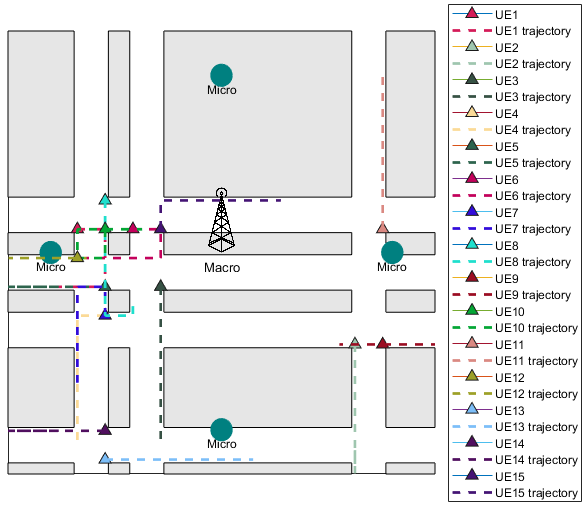
\includegraphics[scale=0.57]{figures/traj.png}
\caption{UEs' trajectories in the urban simulated environment during the final test; green dots represent the micros and the antenna the macro.}\label{img:map} 
\end{figure}
      
%%%%%%%%%%%%%%%%%%%%%%%%%%%%%%%%%%%%%%%%%%%%%%%
\section{Results}\label{sec:res}
%%%%%%%%%%%%%%%%%%%%%%%%%%%%%%%%%%%%%%%%%%%%%%%
\textbf{\textcolor{red}{addressing long term throughput}}The Results section contains a selection of the most relevant results with the explanation of their meaning. Please, not that you do NOT have to describe the shape of the curves that can be seen in the figures, but the reasons WHY such curves have that shape!
%%%%%%%%%%%%%%%%%%%%%%%%%%%%%%%%%%%
\section{Conclusions}\label{sec:conclusion}
%%%%%%%%%%%%%%%%%%%%%%%%%%%%%%%%%%%
Conclusions are a superbrief summary of what has been done and highlighting of the "take home message"
\newpage
\nocite{*}
\bibliographystyle{plain}
\bibliography{biblio}
\end{document}
